% !Mode:: "TeX:UTF-8"
%!TEX program  = xelatex


\documentclass{hitreport}
\usepackage{url}
\usepackage{algorithm}  
\usepackage{algpseudocode}  
\usepackage{amsmath}
\usepackage{cite}
\usepackage{threeparttable}
\usepackage{subfig}
\usepackage{listings} %插入代码
\usepackage{xcolor} %代码高亮
\usepackage{tikz}


\lstset{numbers=left, %设置行号位置
	numberstyle=\tiny, %设置行号大小
	keywordstyle=\color{blue}, %设置关键字颜色
	commentstyle=\color[cmyk]{1,0,1,0}, %设置注释颜色
	frame=single, %设置边框格式
	escapeinside=``, %逃逸字符(1左面的键),用于显示中文
	breaklines, %自动折行
	extendedchars=false, %解决代码跨页时,章节标题,页眉等汉字不显示的问题
	xleftmargin=2em,xrightmargin=2em, aboveskip=1em, %设置边距
	tabsize=4, %设置tab空格数
	showspaces=false %不显示空格
}

\renewcommand{\algorithmicrequire}{\textbf{Input:}}  % Use Input in the format of Algorithm  
\renewcommand{\algorithmicensure}{\textbf{Output:}} % Use Output in the format of Algorithm  

% =============================================
% Part 0 Edit the info
% =============================================

\major{计算机科学与技术}
\name{孙骁}
\title{视听觉信号处理\\课程报告}
\stuid{1180300811} % 学号
\college{计算学部}
\date{2020年10月10日}
\lab{} %实验地点
\course{视听觉信号处理}
\instructor{姚鸿勋}
% \grades{}
\expname{} %实验名称
% \exptype{} % 实验类型
% \partner{} % 同组学生名字
\term{2020秋季学期}

\begin{document}

\maketitle

\tableofcontents
\newpage
\section{信号与系统概述}

\subsection{何为信号}
信号是反映、载有信息的各种物理量,可输入“系统”中进行分析、加工、变换等操作。信号和信息的概念类似,但是信号是信息的表现形式,信息则是信号的具体内容。信号的种类有很多,只要对于系统分析有用的信息,我们都可以将其称为信号,并进行量化分析。采用不同的分类标准可以将信号分为不同的种类,包括确定信号或随机信号、周期信号或非周期信号,但是针对信号与系统的研究,我们主要关心连续时间信号与离散时间信号。

连续时间信号指的是,在某一时间范围内,对于任意时间的函数值,除若干个不连续点之外,都可以给出确定的值;离散时间信号则是离散时间的函数,只在某些不连续的规定瞬间给出函数值,其他时间的函数没有定义。连续时间信号中,有连续幅值和离散幅值的区别,我们也把连续幅值的连续时间信号称为模拟信号;离散时间信号中,连续幅值的信号又被叫做抽样信号,离散幅值的信号是数字信号。

模拟信号可以通过抽样变为抽样信号,再通过量化处理变为数字信号。计算机较适合处理数字信号,通过上述的操作,可以将传感器采集到的信号转化为程序易于处理的信息,便于后续的处理与分析。

\subsection{系统的分类}

不同的系统由于其数学模型的表现形式有所不同,因此有不同的分类方法,常见的分类方法如下:

\begin{enumerate}
\item 线性与非线性系统
\item 时变系统与非时变系统
\item 连续时间系统、离散时间系统和混合系统
\item 即时系统和动态系统
\item 集总参数系统和分布参数系统
\item 因果系统与非因果系统
\item 稳定系统与不稳定系统
\item 可逆系统与不可逆系统
\end{enumerate}

\subsection{信号和系统常见分析方法}

针对不同的信号以及系统,往往采用不同的数学建模方法对实际问题进行建模处理。

\subsubsection{信号的常见分析方法}

连续信号的分析方法有时域分析法和变换域分析法,变换域分析法中常见的是频域下的傅里叶变换分析法和复频域下的拉普拉斯变换分析法。离散信号的分析方法也有时域分析法和变换域分析法,变换域分析法中常见的是离散傅里叶变换分析法和Z变换分析法。

\subsubsection{系统的常见分析方法}
\begin{enumerate}
\item 连续时间系统
\begin{enumerate}
\item 线性非时变系统,使用常系数线性微分方程建模求解;
\item 线性时变系统,使用变参数线性微分方程建模求解;
\item 非线性非时变系统,使用常系数非线性微分方程建模求解;
\item 非线性时变系统,使用变参数非线性微分方程建模求解。
\end{enumerate}
\item 离散时间系统,使用差分方程建模求解。
\end{enumerate}


\section{典型信号及信号的基本运算}

\subsection{典型信号}

\subsubsection{单位矩形脉冲信号}
	\begin{align}\label{equ:Gtaut}
	G_{\tau}\left( t \right) =\left\{ \begin{array}{l}
	1 \ \ \ \ \ ,-\frac{\tau}{2}\le t\le \frac{\tau}{2}\\
	0 \ \ \ \ \ ,\left| t \right|>\frac{\tau}{2}\\
	\end{array} \right.
	\end{align}
其中,$\tau$是矩形脉冲信号的脉冲宽度,由于是单位矩形脉冲信号,则脉冲的高度为1。
\subsubsection{正余弦信号}

正弦信号:$f\left(x\right) = K\sin \left(\omega t+\theta \right)$,余弦信号:$f\left(x\right) = K\cos \left(\omega t+\theta \right)$。其中,$K$是振幅;$\omega$为角频率,与信号的周期有关;$\theta$为初相位。

\subsubsection{指数信号}
连续时间的指数信号为$f\left(t\right) = Ke^{\alpha t} $。当参数$\alpha >0$时,信号增强;当$\alpha <0$时,信号衰减;当$\alpha =0$时,信号为直流信号。指数信号的一个重要特点是,对指数信号求积分或求微分,指数信号的形式保持不变。

\subsubsection{复指数信号}

复指数信号的一般形式为:
\begin{align}\label{equ:Kest}
f\left(t\right) = Ke^{st},
\end{align}
其中,指数因子$s$是复数。而由欧拉公式
\begin{align}\label{equ:ouler}
	\left\{ \begin{array}{l}
	e^{j\omega t} = \cos \omega t + j\sin \omega t\\
	e^{-j\omega t} = \cos \omega t - j\sin \omega t
	\end{array} \right.
\end{align}
\begin{align}
	\left\{ \begin{array}{l}
	\cos \omega t =\frac{e^{j\omega t}+e^{-j\omega t}}{2}\\
	\sin \omega t =\frac{e^{j\omega t}-e^{-j\omega t}}{2j}
	\end{array} \right.
\end{align}
则式(\ref{equ:Kest})可以转化为正余弦信号表示形式:
\begin{align}\label{equ:Kestsin}
f\left(t\right) = \left(Ke^{\sigma t}\cos \omega t\right) +j\left(Ke^{\sigma t}\sin \omega t\right).
\end{align}
从式(\ref{equ:Kestsin})中可以看出,一个复指数信号可以分解成为实、虚两部分。其中,实部包含
余弦信号,虚部则为正弦信号。而且指数因子$\sigma$表示了正弦与余弦信号的振幅随时间变化的情况:若$\sigma > 0$,正弦、余弦信号是增幅振荡;若$\sigma <0$,则正弦、余弦信号是衰减振荡。而指数因子虚部的$\omega$表示正弦与余弦信号的角频率。

\subsubsection{抽样函数}
抽样函数又被称为Sa函数,抽样函数的表达式为:
\begin{align}\label{equ:Sa}
Sa\left(t\right) = \frac{\sin t}{t}
\end{align}
Sa函数有以下特点:
\begin{enumerate}
\item Sa函数为偶函数;
\item Sa函数延t轴两侧振幅递减,且当$t=\pm \pi , \pm 2\pi , \cdots$时,$Sa\left(t\right) = 0$;
\item 
\begin{align}
\left\{ \begin{array}{l}
	\int_{0}^{+\infty}{Sa\left(t\right)d}t = \frac{\pi}{2}\\
	\int_{-\infty}^{+\infty}{Sa\left(t\right)\mathrm{d} t} = \pi
	\end{array} \right.
\end{align}
\end{enumerate}

\subsubsection{高斯信号}
高斯信号表示为:
\begin{align}
f\left(t\right) =  Ke^{-\left(\frac{t}{2}\right)^{2}}.
\end{align}
高斯信号的重要特点是在傅里叶变换后,仍然为高斯函数,保持不变。

\subsubsection{单位冲激信号}

单位冲激函数是,在矩形脉冲宽度为$\tau$,幅度为$\frac{1}{\tau}$时,当$\tau\rightarrow 0$时,脉冲幅度将趋于无限大,矩形脉冲信号在此极限时为单位冲激信号,记为$\delta\left(t\right)$,满足Dirac定义:
\begin{align}
\left\{ \begin{array}{l}
	\int_{-\infty}^{+\infty}{\delta\left(t\right)\mathrm{d}t} = 1\\
	\delta \left(t\right) = 0\ \ \ \ \left(t\ne 0\right)
	\end{array} \right.
\end{align}
单位冲激函数满足很多很有趣的性质:
\begin{enumerate}
\item 抽样性:

设$f\left(t\right)$为连续函数,则
\begin{align}
\left\{ \begin{array}{l}
	\int_{-\infty}^{+\infty}{f\left(t\right)\cdot \delta\left(t\right) \mathrm{d}t} = f\left(0\right)\\
	\int_{-\infty}^{+\infty}{f\left(t\right)\cdot \delta\left(t-t_0\right) \mathrm{d}t} = f\left(t_0\right)
	\end{array} \right.
\end{align}

\item 单位冲激信号的积分为单位阶跃信号,单位阶跃信号的微分等于单位冲激信号;

\item 冲激函数为偶函数,即$\delta\left(t\right) = \delta\left(-t\right)$;

\item 冲激函数的尺度特性满足
\begin{align}
\delta\left(at\right) = \frac{1}{\lvert a\rvert}\delta\left(t\right).
\end{align}

\end{enumerate}


\subsubsection{单位阶跃信号}
单位阶跃信号的表达式为:
\begin{align}
	u\left( t \right) =\left\{ \begin{array}{l}
	1 \ \ \ \ \ ,t>0\\
	0 \ \ \ \ \ ,t<0\\
	\end{array} \right.
\end{align}
在$t=0$处一般无定义,单位阶跃信号也满足一些重要的性质。
\begin{enumerate}
\item 单位阶跃信号的积分为单位斜变信号,即
\begin{align}
R\left(t\right) = \int_{-\infty}^{t}{u\left(\tau\right)\mathrm{d}\tau}
\end{align}

\item 单边特性

任意函数$f\left(t\right)$与$u\left(t\right)$相乘时,使$f\left(t\right)$在跳变点前幅值变为0,跳变点之后的函数保持不变。
\end{enumerate}

\subsubsection{单位斜变信号}

单位斜变信号的表达式为:
\begin{align}
	R\left( t \right) =\left\{ \begin{array}{l}
	t \ \ \ \ \ ,t\ge0\\
	0 \ \ \ \ \ ,t<0
	\end{array} \right.
\end{align}
也有一种特殊的单位斜变信号,是截顶的单位斜变信号,表达式如下:
\begin{align}
	R\left( t \right) =\left\{ \begin{array}{l}
	0 \ \ \ \ \ ,t<0\\
	t \ \ \ \ \ ,0<t<\tau\\
	\tau \ \ \ \ ,t\ge \tau
	\end{array} \right.
\end{align}
单位斜变信号的微分是单位阶跃函数。


\subsubsection{符号函数}

符号函数的定义为:
\begin{align}
	\mathrm{Sgn}\left( t \right) =\left\{ \begin{array}{l}
	1 \ \ \ \ \ ,t>0\\
	-1 \ \ \ \ \ ,t<0\\
	\end{array} \right.
\end{align}
在$t=0$处常常不定义,或定义$\mathrm{Sgn}\left(0\right) = 0$,我们还可以由阶跃函数表示符号函数。
\begin{align}
\mathrm{Sgn}\left(t\right) = u\left(t\right)-u\left(-t\right)
\end{align}

\subsection{信号的基本运算}

\subsubsection{四则远算}
四则远算后的信号,在任意一点的取值定义为原信号在同一点处函数值作相同四则运算的结果。

\subsubsection{反褶运算}
反褶运算定义为$f\left(t\right)\rightarrow f\left(-t\right)$,即,将原信号$f\left(t\right)$的波形按纵轴翻转。

\subsubsection{时移运算}
时移运算定义为$f\left(t\right)\rightarrow f\left(t-b\right)$,其中b决定了平移方向与位移量,当$b>0$时,信号整体右移,当$b<0$时,信号整体左移,时移运算的通俗解释是,将原信号$f\left(t\right)$的波形沿横轴平移b个单位。

\subsubsection{压扩运算}

压扩运算又被称为尺度变换,变换方法为$f\left(t\right)\rightarrow f\left(at\right)$。当$a>0$时,信号的波形不需要反褶,当$a<0$时,信号的波形需要反褶;当$\lvert a\rvert>1$时,信号的波形会被压缩,当$\lvert a \rvert<1$时,信号的波形会被扩张,倍数为$\left. 1 / \right. {\lvert a\rvert}$。

\subsubsection{卷积运算}
卷积运算的定义为:
\begin{align}
f_{1}\left(t\right) \ast f_{2}\left(t\right) = \int_{-\infty}^{+\infty}{f_{1}\left(\tau\right) f_{2}\left(t-\tau \right) \mathrm{d}\tau}
\end{align}
卷积运算满足很多性质:
\begin{enumerate}
\item 交换律,$f_1 \ast f_2 = f_2 \ast f_1$;
\item 分配律,$f_1 \ast \left(f_2+f+3\right) = f_1 \ast f_2+f_1 \ast f_3$,此条性质常用于并联系统的分析;
\item 结合律,$f_1 \ast \left(f_2 \ast f_3\right) = \left(f_1 \ast f_2\right)\ast f_3$,此条性质常用于串联系统的分析;
\item 函数与单位冲激函数的卷积,相当于将该函数平移到单位冲激函数的冲击点的位置,这也是冲激函数的搬移特性。
\begin{align}
f\left(t\right) \ast \delta \left(t-t_0\right) = f\left(t-t_0\right)
\end{align}

\item 卷积的积分性质:两个信号卷积的积分等于其中任一信号的积分与另一信号的卷积,即
\begin{align}
\int_{-\infty}^{t}{\left(f_1 \ast f_2\right)\left(\lambda\right)\mathrm{d}\lambda} = f_1\left(t\right) \ast \left[\int_{-\infty}^{t}f_2\left(\lambda\right)\mathrm{d}\lambda\right] =  \left[\int_{-\infty}^{t}f_1\left(\lambda\right)\mathrm{d}\lambda\right] \ast f_2\left(t\right)
\end{align}

\item 卷积的微分性质:两个信号卷积的微分等于其中任一信号的微分与另一信号的卷积,即
\begin{align}
\frac{\mathrm{d} }{\mathrm{d} t}{\left[f_1\left(t\right) \ast f_2\left(t\right)\right]} = f_1\left(t\right) \ast \left[\frac{\mathrm{d} }{\mathrm{d} t}f_2\left(t\right)\right] = \left[\frac{\mathrm{d} }{\mathrm{d} t}f_1\left(t\right)\right]\ast f_2\left(t\right)
\end{align}

\item 由上两条性质,拓展得到卷积运算的高阶导数与多重积分间的规律。
\begin{align}
\left(f_1 \ast f_2\right)^{n}\left(t\right) = f_1^{m}\left(t\right) \ast f_2^{n-m}\left(t\right)
\end{align}
上式中,m,n,n-m取正整数时为导数阶次,取负数时为积分次数。

\end{enumerate}

\subsubsection{相关运算}
相关运算的定义为:
\begin{align}\label{equ:xiangguan1}
R_{f_{1}f_{2}}\left(t\right) = R\left(f_1\left(t\right), f_2\left(t\right)\right) = \int_{-\infty}^{+\infty}{f_1\left(\tau \right) f_{2}^{*}\left(\tau -t\right) \mathrm{d}\tau} = \int_{-\infty}^{+\infty}{f_1\left(\tau +t\right) f_{2}^{*}\left(\tau\right) \mathrm{d}\tau}
\end{align}
\begin{align}\label{equ:xiangguan2}
R_{f_{2}f_{1}}\left(t\right) = R\left(f_2\left(t\right), f_1\left(t\right)\right) = \int_{-\infty}^{+\infty}{f_2\left(\tau \right) f_{1}^{*}\left(\tau -t\right) \mathrm{d}\tau} = \int_{-\infty}^{+\infty}{f_2\left(\tau +t\right) f_{1}^{*}\left(\tau\right) \mathrm{d}\tau}
\end{align}
其中$f_{1}^{*}\left(\tau -t\right)$由$f_1$的负数共轭并反褶平移后得到,由式(\ref{equ:xiangguan1})与式(\ref{equ:xiangguan2}) 可知,$R_{f_1f_2}\left(t\right) = R_{f_2f_1}^{*}\left(-t\right)$,相关运算与函数的次序有关。
并且我们可以得到相关运算与卷积的关系:
\begin{align}
R_{f_2f_1}\left(t\right) = f_{1}^{*}\left(-t\right) \ast f_2\left(t\right)
\end{align}
实际上,在图像处理的卷积运算中,卷积运算和相关运算的差异位卷积核是否旋转$180°$,旋转$180°$即为卷积操作,不旋转$180°$即为相关操作。

相关运算的另一个主要应用时自相关,即函数自身求相关。
\begin{align}
R_f\left(t\right) = \int_{-\infty}^{+\infty}{f\left(t\right) f^{*}\left(\tau -t\right)\mathrm{d}\tau} = \int_{-\infty}^{+\infty}{f\left(\tau+t\right)f^{*}\left(\tau\right)\mathrm{d} \tau}
\end{align}
我们可以发现:
\begin{enumerate}
\item 实函数的自相关是偶函数;
\item 周期函数的相关函数总是在周期的整数倍nT处取得最大值。
\end{enumerate}

\section{信号分解}

信号分解是信号处理的一个重要方法,通过对信号的分解,可以将复杂的信号分解成多个简单的信号,通过研究已知的简单信号的性质来对复杂信号进行分析,这个是一种“降维”的思想,将复杂问题分解成简单的问题,通过依次分析解决简单的问题来分析复杂问题。
信号常见的分解方式如下:
\begin{enumerate}
\item 直流交流分解
\item 奇偶分解
\item 实部虚部分解
\item 脉冲分解
\item 正交分解
\end{enumerate}

\subsection{直流交流分解}
直流交流分解是将信号分解出直流分量与交流分量,直流分量为信号一个周期内的均值,若信号为非周期信号,即为信号的均值。所以定义
\begin{align}
\left\{ \begin{array}{l}
	\text{直流分量}\ \ \ f_{DC}\left(t\right) = \underset{T\rightarrow \infty}{\lim}\frac{1}{T}\int_{-\frac{T}{2}}^{\frac{T}{2}}{f\left( t \right) \mathrm{d}t}\\
	\text{交流分量}\ \ \ f_{AC}\left(t\right) = f\left(t\right) - f_{DC}\left(t\right)
	\end{array} \right.
\end{align}

\subsection{奇偶分解}
任何函数均可被分解成奇函数与偶函数的和,同理信号也可以被分解成奇分量和偶分量。
\begin{align}
\left\{ \begin{array}{l}
	f_{e}\left(t\right) = Ev\left[f\left(t\right)\right] = \dfrac{f\left(t\right)+f\left(-t\right)}{2}\\
	f_{o}\left(t\right) = Od\left[f\left(t\right)\right] = \dfrac{f\left(t\right)-f\left(-t\right)}{2}
	\end{array} \right.
\end{align}

\subsection{实部虚部分解}
任何信号也可以被分解成实部分量与虚部分量,即:
\begin{align}
\left\{ \begin{array}{l}
	f_{e}\left(t\right) = \textbf{Re}\left[f\left(t\right)\right] = \dfrac{f\left(t\right)+f^{*}\left(t\right)}{2}\\
	f_{i}\left(t\right) = \textbf{Im}\left[f\left(t\right)\right] = \dfrac{f\left(t\right)-f^{*}\left(t\right)}{2j}
	\end{array} \right.
\end{align}

\subsection{脉冲分解}
信号可以近似地表示为一组矩形脉冲的和的形式,信号被分解后,$t_1$处宽度为$\Delta t_1$的矩形脉冲可表示为
\begin{align}
f_{t_1}\left(t\right) = f\left(t_1\right)\left[u\left(t-t_1\right)-u\left(t-t_1-\Delta t_1\right)\right],
\end{align}
则原函数可以表示为
\begin{align}
f\left(t\right) \approx \sum_{t=-\infty}^{+\infty}{f_{t_1}\left(t\right)}
\end{align}


\section{正交分解}

正交分解是信号分析中最常用的方法,既满足了分解信号化繁为简的要求,也通过正交分解的唯一性获得了信号在新的欧式空间中的唯一表示。通过正交分解与空间投影变换,我们可以将信号映射到一个新的空间中,在新的空间中研究信号的性质,并通过空间变换的映射获得信号在多种不同表示空间中的对应关系。

最早接触正交分解是在线性代数中,通过选择高维空间中的一组基底,可以将高维空间中的每一个向量唯一表示。而学习了信号与系统之后,知晓了函数也可以通过选择正交的基底函数进行正交分解。但是无论是向量的正交分解还是函数的正交分解,都是使用易于研究的分量将高维的向量或函数线性表示,从而简化分析。

\subsection{向量的正交分解}

信号的频域分解与向量的分解十分类似,在中学的物理学习过力的分解与合成,其需要符合平行四边形法则,如图(\ref{fig:F})所示,可以看到,力的分解不唯一,在不同方向上分解,结果是不同的。
\begin{figure}[H]
\centering
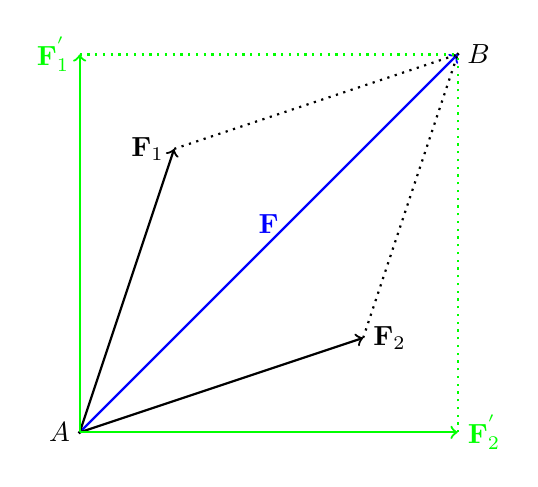
\begin{tikzpicture}[scale=1.2]

\coordinate[label = left: $A$] (A) at (0, 0);
\coordinate[label = right: $B$] (B) at (4, 4);
\node at (A)[circle,fill,inner sep=0.5pt]{};
\node at (B)[circle,fill,inner sep=0.5pt]{};

\draw[blue,thick,->] (0,0) -- (4,4) node[above, midway] (line) {$\textbf{F}$};
\draw[black,thick,->] (0,0) -- (1,3) node[left] (line) {$\textbf{F}_1$};
\draw[black,thick,->] (0,0) -- (3,1) node[right] (line) {$\textbf{F}_2$};
\draw[black,thick, dotted] (1,3) -- (4,4) node[above, midway] (line) {};
\draw[black,thick, dotted] (3,1) -- (4,4) node[above, midway] (line) {};
\draw[green,thick,->] (0,0) -- (0,4) node[left] (line) {$\textbf{F}_{1}^{'}$};
\draw[green,thick,dotted] (0,4) -- (4,4) node[above, midway] (line) {};
\draw[green,thick,->] (0,0) -- (4,0) node[right] (line) {$\textbf{F}_{2}^{'}$};
\draw[green,thick,dotted] (4,0) -- (4,4) node[above, midway] (line) {};

\end{tikzpicture}
\caption{力的合成与分解}\label{fig:F}
\end{figure}

将力抽象成向量,在平面上的一个向量$\textbf{A}_0$,可以在两个方向$\textbf{A}_1$,$\textbf{A}_2$上分解。分解方式选择不唯一,分解的结果也不唯一。

推广至更一般的向量空间,我们有如下定理:
\begin{theorem}
令\textit{H}是n维向量空间\textit{V}的一个子空间,\textit{V}中向量的指标集$\mathcal{B} = \left\{\textbf{b}_1,\cdots,\textbf{b}_n\right\}$称为\textit{H}的一组基底,如果:
\begin{enumerate}
\item $\mathcal{B}$是一线性无关集.
\item 由$\mathcal{B}$生成的子空间与\textit{H}相同,即$\textit{H} = \text{Span}\left\{\textbf{b}_1,\cdots,\textbf{b}_n\right\}$.
\end{enumerate}
\end{theorem}

如果$\textbf{b}_1,\cdots,\textbf{b}_n$之间相互正交,则称其是正交基,如果在\textit{n}维向量空间中的任意一个向量可以用$\textbf{b}_1,\cdots,\textbf{b}_n$这组基底的线性组合表示,则称这组基底是完备的。于是我们得到,\textit{n}维向量空间中的任何一个向量都可以由选定的正交完备基底线性表示,并且这种表示是唯一的。也就是说,\textit{n}维向量空间中的任何向量,均可分解成基底的线性组合。这也说明了向量分解的平行四边形法则的正确性。

\subsection{信号的正交分解}

由向量空间的基底的定义可知,如果我们想分解由函数表示的信号,也必须在函数的空间中找到函数空间的“基底”,使用这组“基底”将目标函数线性表示出来,由于函数不能做类似向量一样的内积运算,因此我们首先引入正交函数的概念,并定义函数何为正交。
\begin{description}
\item[正交函数] 

若在区间$\left(t_1,t_2\right)$上,函数$f_1\left(t\right)$与函数$f_2\left(t\right)$互不含有对方的分量,则称$f_1\left(t\right)$与函数$f_2\left(t\right)$在$\left(t_1,t_2\right)$上正交。
\end{description}
\begin{theorem} [函数正交的充要条件]
函数正交的充要条件是函数的内积为0,即
\begin{align}
\left< f_1,f_2\right> = \int_{t_1}^{t_2}{f_1\left(t\right)f_2\left(t\right)\mathrm{d}t} = 0
\end{align}
\end{theorem}

因此,在函数空间中选择的互相正交的函数,类似于向量空间中选择的基底,当我们在区间$\left(t_1,t_2\right)$选择一组完备的正交函数集时,任意函数$f\left(t\right)$在区间$\left(t_1,t_2\right)$上可表示为正交函数集内函数的线性组合,即
\begin{align}
f\left(t\right) = \sum_{n=1}^{N}{c_ng_n\left(t\right)}\ \ \ \ c_n\text{为正交系数分量}
\end{align}

常见的正交分解变换有:
\begin{enumerate}
\item 傅里叶变换
\item 离散余弦变换
\item Walsh-Hadamard 变换
\item 斜变换
\item Haar 变换
\item 离散小波变换
\item 离散K-L变换
\item 奇异值分解SVD变换
\item Z变换 
\end{enumerate}

下面主要介绍傅里叶变换和Z变换,并针对二者适用的不同范围做分析总结。

\subsection{傅里叶变换}
傅里叶变换常用于连续时间信号与系统的频域分析,其将一个非周期信号$f\left(t\right)$分解为在时域和频域中都连续的指数函数$e^{j\omega t}$,而通过欧拉公式(\ref{equ:ouler})可以得到正弦余弦形式的傅里叶变换公式。我们主要关心一维连续傅里叶变换的性质与二维离散傅里叶变换的性质。

\subsubsection{一维连续傅里叶变换}

令$f\left(t\right)$为实变量\textit{x}的连续函数,$f\left(x\right)$的傅里叶变换与傅里叶反变换定义如下:
\begin{description}
\item[一维连续傅里叶变换] 
一维连续傅里叶变换定义如下:
\begin{align}
\mathscr{F}\left\{f\left(x\right)\right\} = \int_{-\infty}^{+\infty}f\left(t\right) e^{-j2\pi ux} \mathrm{d}x = F\left(u\right)
\end{align}
\end{description}

\begin{description}
\item[一维连续傅里叶反变换] 

一维连续傅里叶反变换定义如下:
\begin{align}
\mathscr{F}^{-1}\left\{F\left(u\right)\right\} = \int_{-\infty}^{+\infty}{F\left(u\right)e^{j2\pi ux}\mathrm{d} u} = f\left(x\right)
\end{align}
\end{description}

\subsubsection{一维连续傅里叶变换的性质}
\begin{enumerate}
\item 在振幅谱图中,亮度正比于$\lvert F\left(u,v\right) \rvert$
\item 对称性

傅里叶变换的对称性列表
\begin{enumerate}
\item 偶分量函数在变换中产生偶分量函数;
\item 奇分量函数在变换中产生奇分量函数;
\item 奇分量函数在变换中引入系数$-j$;
\item 偶分量函数在变换中不引入系数。
\end{enumerate}
\item 虚实分量变化

在傅里叶变换中,
\begin{enumerate}
\item 实偶部产生一个实偶部分;
\item 实奇部产生一个虚奇部分;
\item 虚偶部产生一个虚偶部分;
\item 虚奇部产生一个实奇部分。
\end{enumerate}
\item 加法原理

在时域或空域中保持的加法,在频域下也成立,即如果满足$\mathscr{F}\left\{f\left(x\right)\right\} = F\left(u\right)$和$\mathscr{F}\left\{g\left(x\right)\right\} = G\left(u\right)$,则有$\mathscr{F}\left\{f\left(x\right)+g\left(x\right)\right\} = F\left(u\right)+G\left(u\right)$。

\item 平移原理

函数平移不改变其傅里叶变换后的幅值,只改变其实部和虚部间的能量分布。即
\begin{align}
\mathscr{F}\left\{f\left(x-a\right)\right\} &= \int_{-\infty}^{+\infty}{f\left(x-a\right)e^{-j2\pi ux}\mathrm{d} x}\\
&=e^{-j2\pi ua}F\left(u\right)
\end{align}

\item 卷积定理

卷积定理在傅里叶变换下满足如下性质:
\begin{align}
\left\{ \begin{array}{l}
	\mathscr{F}\left\{f\left(x\right)\ast g\left(x\right)\right\} = F\left(u\right)G\left(u\right)\\
	\mathscr{F}^{-1}\left\{F\left(u\right)G\left(u\right)\right\} = f\left(x\right)\ast g\left(x\right)
	\end{array} \right.
\end{align}

\item 相似性原理

当对$f\left(x\right)$做伸缩变换时,满足
\begin{align}
\mathscr{F} \left\{f\left(ax\right)\right\} = \frac{1}{\lvert a \rvert}F\left(\frac{u}{a}\right)
\end{align}

\item 能量守恒

在傅里叶变换前后,信号的能量保持不变,有
\begin{align}
E=\int_{-\infty}^{+\infty}{\lvert f\left(x\right) \rvert^{2}\mathrm{d}x} = \int_{-\infty}^{+\infty}{\lvert F\left(u\right) \rvert^{2}\mathrm{d}u}
\end{align}
\end{enumerate}

\subsubsection{一维离散傅里叶变换}

\begin{description}
\item[一维离散傅里叶变换] 

定义一维离散傅里叶变换如下:
\begin{align}
F\left(u\right) = \frac{1}{N}\sum_{i=0}^{N-1}{f\left(i\right)e^{\left. -j2\pi ui / N \right.}},\ \ \ \ u=0,1,2,\cdots,N-1
\end{align}
\end{description}
\begin{description}
\item[一维离散傅里叶反变换] 

定义一维离散傅里叶反变换如下:
\begin{align}
f\left(i\right) = \sum_{u=0}^{N-1}{F\left(u\right)e^{\left. j2\pi ui / N \right.}},\ \ \ \ i=0,1,2,\cdots,N-1
\end{align}
\end{description}



\subsubsection{二维连续傅里叶变换}

\begin{description}
\item[二维傅里叶变换] 
定义$f\left(x,y\right)$的傅里叶变换如下:
\begin{align}
\mathscr{F} \left\{f\left(x,y\right)\right\} = \int_{-\infty}^{+\infty}\int_{-\infty}^{+\infty}{f\left(x,y\right)e^{-j2\pi \left(ux+vy\right)} \mathrm{d}x\mathrm{d}y} = F\left(u,v\right)
\end{align}
\end{description}

\begin{description}
\item[二维傅里叶变换] 
定义$F\left(u,v\right)$的傅里叶反变换如下:
\begin{align}
\mathscr{F}^{-1} \left\{F\left(u,v\right)\right\} = \int_{-\infty}^{+\infty}\int_{-\infty}^{+\infty}{F\left(u,v\right)e^{j2\pi \left(ux+vy\right)} \mathrm{d}u\mathrm{d}v} = f\left(x,y\right)
\end{align}
\end{description}

\subsubsection{二维离散傅里叶变换}

\begin{description}
\item[二维离散傅里叶变换] 

定义二维离散傅里叶变换如下:
\begin{align}
F\left(u,v\right) = \frac{1}{MN}\sum_{x=0}^{M-1}\sum_{y=0}^{N-1}{f\left(x,y\right)e^{-j2\pi \left(\frac{ux}{M}+\frac{vy}{N}\right)}},\ \ \ \ 
\left\{ \begin{array}{l}
u=0,1,2,\cdots,M-1\\
v = 0,1,2,\cdots,N-1	
\end{array}\right.
\end{align}
\end{description}
\begin{description}
\item[二维离散傅里叶反变换] 

定义二维离散傅里叶反变换如下:
\begin{align}
f\left(x,y\right) = \sum_{u=0}^{M-1}\sum_{v=0}^{N-1}{F\left(u,v\right)e^{j2\pi \left(\frac{ux}{M}+\frac{vy}{N}\right)}},\ \ \ \ 
\left\{ 
\begin{array}{l}
x=0,1,2,\cdots,M-1\\
y = 0,1,2,\cdots,N-1	
\end{array}
\right.
\end{align}
\end{description}

\subsubsection{二维离散傅里叶变换性质}

\begin{enumerate}
\item 可分离性

可以将二维傅里叶变换拆分成两个部分,变为两个一维部分进行处理。
\begin{align}
\left\{
\begin{array}{l}
F\left(u,v\right) = \dfrac{1}{M}\sum\limits_{x=0}^{M-1}{e^{\left. -j2\pi ux / M\right.}}\cdot \dfrac{1}{N}\sum\limits_{y=0}^{N-1}{f\left(x,y\right)e^{\left. -j2\pi vy / N\right.}}\\
f\left(x,y\right) = \sum\limits_{u=0}^{M-1}{e^{\left. j2\pi ux / M \right.}}\sum\limits_{v=0}^{N-1}{F\left(u,v\right) e^{\left. j2\pi vy / \right.}}	
\end{array}
\right.
\end{align}

\item 线性性质

二维离散傅里叶变换满足

\begin{align}
\mathscr{F}\left\{af\left(x,y\right)+bg\left(x,y\right)\right\} = a\mathscr{F}\left\{f\left(x,y\right)\right\}+b\mathscr{F}\left\{g\left(x,y\right)\right\}
\end{align}

\item 比例性

二维离散傅里叶变换的比例性质为

\begin{align}
\mathscr{F}\left\{af\left(x,y\right)\right\} = a\mathscr{F}\left\{f\left(x,y\right)\right\} = aF\left\{u,v\right\}
\end{align}
\begin{align}
\mathscr{F}\left\{f\left(ax,by\right)\right\} = \dfrac{1}{\lvert ab \rvert}F\left(\dfrac{u}{a},\dfrac{v}{b}\right)
\end{align}

\item 卷积定理

二维离散傅里叶变换满足
\begin{align}
f\left(x,y\right)\ast g\left(x,y\right) = \sum\limits_{m=0}^{M-1}\sum\limits_{n=0}^{N-1}{f\left(m,n\right)g\left(x-m,y-n\right)}
\end{align}
\begin{align}
\mathscr{F}\left\{f\left(x,y\right)\ast g\left(x,y\right)\right\} = F\left(u,v\right)G\left(u,v\right)
\end{align}

\end{enumerate}


\subsection{Z变换}

因为傅里叶变换不会对所有序列均收敛,所以引入应用更广泛的Z变换,Z变换时将离散系统的差分方程变换为代数方程,类似于连续时间信号的Lapalce变换。也即离散时间信号的Z变化和连续时间信号的Lapalce变换互相对应。

\subsubsection{Z变换定义}

任意序列$x\left(n\right)$的离散时间傅里叶变换为
\begin{align}
X\left(e^{j\omega}\right) = \sum\limits_{n=-\infty}^{+\infty}{x\left(n\right)e^{-j\omega n}}
\end{align}
则序列$x\left(n\right)$的Z变换$X\left(z\right)$定义为
\begin{align}
X\left(z\right) = \mathscr{Z}\left\{x\left(n\right)\right\}=\sum\limits_{n=-\infty}^{+\infty}x\left(n\right)z^{-n}
\end{align}

\subsubsection{Z变换的性质}

\begin{enumerate}
\item 线性性质

若$x\left(n\right)$的Z变换为$X\left(z\right)$,$y\left(n\right)$的Z变换为$Y\left(z\right)$,则
\begin{align}
\mathscr{Z}\left\{ax\left(n\right)+by\left(n\right)\right\} = aX\left(z\right)+bY\left(z\right)
\end{align}

\item 时移性

若$x\left(n\right)$的Z变换为$X\left(z\right)$,则
\begin{align}
\mathscr{Z}\left\{x\left(n-m\right)\right\} = z^{-m}X\left(z\right)
\end{align}

\item Z域微分性质

若$x\left(n\right)$的Z变换为$X\left(z\right)$,则
\begin{align}
\mathscr{Z}\left\{nx\left(n\right)\right\} = -z\dfrac{\mathrm{d}\left[X\left(z\right)\right]}{\mathrm{d}z}
\end{align}

\item 终值定理

若$x\left(n\right)$的Z变换为$X\left(z\right)$,则
\begin{align}
\underset{n\rightarrow \infty}{\lim}x\left(n\right) = \underset{n\rightarrow \infty}{\lim}\left[\left(z-1\right)X\left(z\right)\right]
\end{align}
\end{enumerate}

\subsection{信号正交分解的理解}

其实无论是傅里叶变换亦或是Z变换,都是为了将信号从时域转化为复域或频域进行表示,并在新的坐标系下对信号进行研究,获得在新坐标系下信号的性质。

信号的正交分解类似于向量在线性空间中的表示方法,线性空间中的基底对应于信号正交分解的完备正交函数集,而基底将向量在线性空间中唯一表示对应于使用完备正交函数集中的函数线性表示其他函数。傅里叶级数的完备正交函数集为$$\left\{1,\sin\left(n\omega t\right),\cos\left(n\omega t\right)\right\},$$这三个函数在一个周期$\left(t_0,t_0+T\right)$内满足完备正交函数集的定义,所以我们可以使用完备正交函数集中的函数将$\left(t_0,t_0+T\right)$内的函数线性表示,因此我们得到了使用傅里叶级数对周期信号进行正交分解的定理:
\begin{theorem}
对任意周期为T,角频率为$\frac{2\pi}{T}$的周期信号$f\left(t\right)$,若满足$\int_{i\infty}^{+\infty}{\lvert f\left(t\right) \rvert\mathrm{d}t}<\infty$,则可以做如下分解:
\begin{align}
f\left(t\right) &=\dfrac{a_0}{2}+a_1\cos \left(\omega t\right)+b_1\sin \left(\omega t\right)+a_2\cos \left(2\omega t\right)+b_2\sin \left(2\omega t\right)\\
& \ \ \ \ \ \ +\cdots+a_n\cos \left(n\omega t\right)+b_n\sin \left(n\omega t\right)\\
&=\dfrac{a_0}{2}+\sum\limits_{n=1}^{+\infty}\left[a_n\cos \left(n\omega t\right)+b_n\sin \left(n\omega t\right)\right]
\end{align}
\end{theorem}

从中我们可以看到,确实可以使用完备正交函数集$\left\{1,\sin\left(n\omega t\right),\cos\left(n\omega t\right)\right\}$内的函数将周期函数唯一表示,但是这个级数有无穷项,在实际问题中常常截断到某一精度,所以不能十分精确的表示一个周期信号,并且使用傅里叶级数分解的条件较为苛刻,要求满足Dirichlet条件。但是傅里叶级数提供了一种表达函数的新思路,使用不同周期的正余弦信号表示周期信号,这里用到了一种投影变换的思想,正常我们熟知的函数信号表示方法是基于xy坐标系的,而傅里叶级数分解将函数放在了正余弦的空间中,也能将函数唯一表示,并且将函数的“主次矛盾”进行了分解,“主要矛盾”即周期大的正余弦信号,“次要矛盾”即周期小的正余弦信号,我们在舍弃周期较小的级数时也是忽略了对函数影响较小的“次要矛盾”,所以通过傅里叶级数分解可以有效提取信号的主要特征,减小次要矛盾对系统分析的影响。譬如在图像处理中,通过对图像的傅里叶变换,对其幅值图像的某一或某些特定频率进行处理,再通过反变换还原,可以得到在时域下滤波的效果。

虽然傅里叶变换可以将信号的主次矛盾分得清楚,上述文段也提到了,使用傅里叶变换的条件较为苛刻,并不是所有的信号都满足Dirichlet条件,因此引入了Z变换。

Z变换在时域序列的基础上乘了一个$z^{-n}$,通过选取合适的$z$,可以使得乘积$x\left(n\right)z^{-n}$收敛,因此解决了傅里叶变换不能对所有序列收敛的问题,Z变换主要应用于离散时间信号,因为其的方法类似于连续时间信号下的Lapalce变换,所以限制也更少,性质也类似于Lapalce变化,Z变换在图像处理领域的主要应用是消除匀速直线运动模糊。在信号与系统的分析中,Z变换可以将差分方程转化为代数方程求解,求解的一般思路是通过对差分方程做Z变换得到代数方程,求解代数方程后再使用逆Z变换得到系统输入的全响应。


\section{空间投影变换}

前文也提到,傅里叶变换将时域下的信号在频域下唯一表示,变换了表示空间,这里用到了变换坐标系的思想,也就是空间放射变换。最早接触变换坐标系是在解线性方程组的时候,当线性方程组有无数组解的时候,我们需要在其对应的线性方程组中找到一个特解,并在其对应的非线性方程组中找到一组极大线性无关组,通过这两部分可以拼接得到最终的解向量。但是极大线性无关组在一个向量空间中并不唯一,当我们使用一组极大线性无关组去表示同一线性空间中的另一组极大线性无关组时,需要乘的系数矩阵即为Jacobi矩阵。

Jacobi矩阵的主要应用在空间投影变换,变换坐标系时,“旧坐标系”和“新坐标系”相关联的那个系数矩阵。比较经典的应用就是在二重积分中,当我们对积分变量做线性变换时,因为积分变量的改变,我们需要乘一个系数矩阵,这个就是空间投影变换的核心。下面给出空间投影变换的介绍。

\paragraph{投影变换}

投影变换是指将原函数在新的坐标系下表示的一种变换方法,在信号处理领域主要是将信号在不同的空间进行表示,这样可以根据坐标系选择感兴趣的信息进行提取。在图像处理的领域,用三维空间的投影变换举例,往往对应式(\ref{equ:change})的对应关系。
\begin{align}\label{equ:change}
\left( \begin{array}{l}
	x\\
	y\\
	z\\
\end{array} \right) =\left( \begin{matrix}
	a_{11}&		a_{12}&		a_{13}\\
	a_{21}&		a_{22}&		a_{23}\\
	a_{31}&		a_{32}&		a_{33}\\
\end{matrix} \right) \left( \begin{array}{l}
	u\\
	v\\
	1\\
\end{array} \right) 
\end{align}
于是我们有对应的坐标对应关系:
\begin{align}
\left\{ \begin{array}{l}
x = a_{11}u+a_{12}v+a_{13}\\
y = a_{21}u+a_{22}v+a_{23}\\
z = a_{31}u+a_{32}v+a_{33}
\end{array}
\right.
\end{align}

投影变换将一个四边形区域内的点投影到另一个四边形中,通过矩阵乘法实现线性变换,与仿射变换不同的是,投影变换也实现了线性变换和平移,相当于在将原图像进行了伸缩变换。以上公式中,设变换之前的点是$z$值为1的点,它三维平面上的点是$\left(x,y,1\right)$,在二维平面上的投影是$\left(x,y\right)$,通过矩阵变换成三维中的点$\left(x,y,z\right)$,再通过除以三维中Z轴的值,转换成二维中的点。从以上公式可知,仿射变换是透视变换的一种特殊情况,它把二维转到三维,变换后,再转映射回之前的二维空间。变换完成后,相当于对图像做了相应的变换。

\section{总结}

《视听觉信号处理》课程的第一部分主要是介绍信号与信号的分析方法,是之后的图像、音频处理的基础,总结了这一阶段的主要知识点,并对本章节重要的两部分:信号的正交分解与空间投影变换做了简要的分析,加入了自己的一些理解,串联了之前线性代数的知识,其实这些思想之前一直都有接触,但是从旧知识中提取思想,并将其运用在新的知识点上,也有不一样的收获,使用已有知识去解释新知识,也是一种便于理解的好方法。

\renewcommand\refname{参考文献}
 
\begin{thebibliography}{2}
\bibitem{book:li}
张晔, 《信号与系统》(第四版).

\bibitem{book:zhou}
David C. Lay; Steven R. Lay; Judi J. McDonald; Linear Algebra and Its Applications (Fifth Edition).
\end{thebibliography}


\end{document}
